\documentclass[../../main.tex]{subfiles}

\begin{document}

A system architecture is the conceptual model that defines the structure, behavior, and more views of a system. An architecture description is a formal description and representation of a system, organized in a way that supports reasoning about the structures and behaviors of the system. The purpose of system architecture activities is to define a comprehensive solution based on principles, concepts, and properties logically related to and consistent with each other.

\begin{figure}[H]
    \centering
    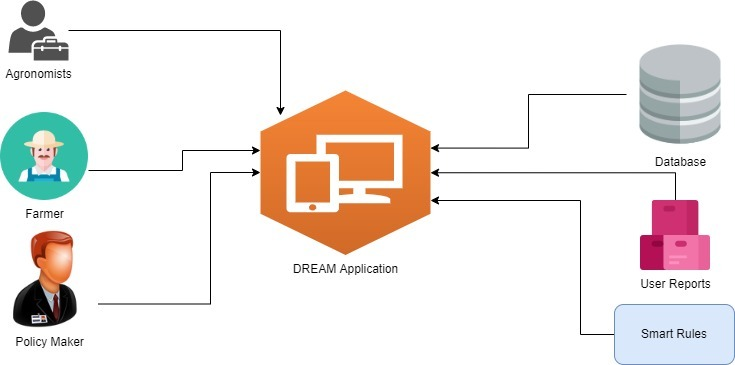
\includegraphics[width=\textwidth]{Architecture.jpeg}
\end{figure}

The below architecture of DREAM application shows three layers of the system the first is the presentation layer which contains the interaction between system users and the interface of the system. The second layer of the architecture is business layer which represents the web server containing application features system is offering. The third layer is the data access layer for the system database to store all the system information. The three main users of the system are policy makers, farmers and agronomists. 


\begin{figure}[H]
    \centering
    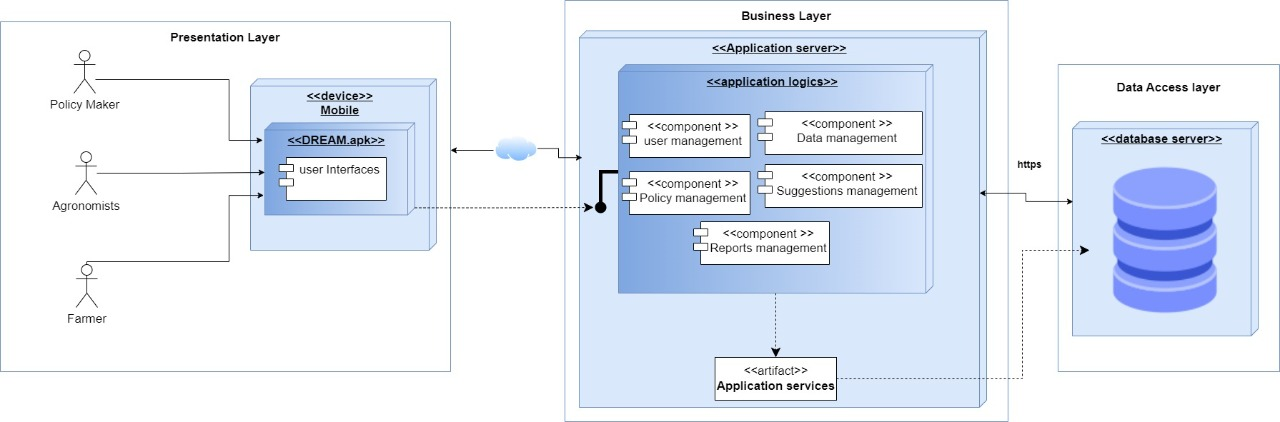
\includegraphics[width=\textwidth]{3_tier_architecture.jpeg}

\end{figure}

\end{document}
